%!TEX root = ../../dissertation.tex
%%%%%%%%%%%%%%%%%%%%%%%%%%%%%%%%%%%%%%%%%%%%%%%%%%%%%%%%%%%%%%%%%%%%%%%%%%%%%%%%
\chapter{Video Streaming Techniques}
\label{chap:streaming}

This chapter is structured as follows.

\begin{itemize}
\item Introduction. Streaming, Popularity. Chapter Intention.
\item Technical Background. Reliable and Unreliable Streaming. Realtime and Stored Streaming.
\item Protocol Overview. Transport and Application Layer. Adaptive Streaming
\item Metrics for Streaming Evaluation. Differences 
\item Models for reliable (adaptive) Streaming
\item Streaming Measurements
\item Summary
\end{itemize}


%%% FITCE intro
Web-based video delivery uses the Web's general purpose transfer protocols, primarily HTTP and the underlying TCP transport protocol. The only requirement to participate in this form  of video streaming is either a recent version of one's favorite web browser supporting the HTML5 \texttt{<video>} tag or, becoming less important, a player for Flash content. This user-friendliness opened the curtains for a much broader audience when compared to RTP streaming approaches. Popular examples include sites with user generated content like YouTube which has an especially large number of viewers and high watch duration \cite{comscore2011ranking}, and commercial sites such as Netflix and Hulu. Netflix accounts for 30\% of today's peak downstream Internet traffic in North America \cite{sandvine_spring2011}, also demonstrating the huge demand for this type of service.

The proportion of total Internet traffic shifted hugely towards video transfers in recent years. Google, who operates YouTube since 2006, now carries a large percentage of that traffic \cite{nw2010carrier}. But the Internet's traffic volume is expected to continue to rise in the next years. If the underlying network infrastructure is not upgraded at the the same speed, this could result in performance degradations for the Internet. Moreover, mobile networks struggle with limited and shared bandwidths, high delay and considerable loss due to intrinsic radio problems, even with new and upcoming mobile specifications such as LTE. Web-based video delivery does not use specialized streaming techniques such as quality scaling, loss tolerance or dedicated signaling connections, but still needs to be able to work well even under theses circumstances

This paper investigates how Web-based media delivery works in general, and how meaningful measurement of its streaming quality can be achieved with future network developments and degraded network parameters in mind.



%% PV intro
Video streaming resonates well with web users, and streaming traffic makes up an ever-growing share of network traffic. At the same time, multiple streaming methods exists, resulting in a multitude of protocols, codecs, and their variety increases at an astonishing rate. Furthermore, the current boom in smart-phones creates an increasing plurality of access network technologies across which media are streamed.

This poses a problem to traditional analytical approaches like source-traffic modeling: Such models are complex to develop, and hard to adapt to new streaming mechanisms; often, they deliberately omit details for reasons of analytical tractability, or only look at single layers of the network stack.

The method presented in this paper rather aims to evaluate performance by capturing generic behavioral patterns of streaming mechanisms, embracing the perspective of a streaming application. Specifically, we model the level of the playback buffer, and thus can subsume both network and playback behavior, while maintaining flexibility and adaptability with regards to the actual streaming server implementation, type of transmission network, protocol stack, and codec. Our model reports perceivable artefacts of buffer underruns, e.g. skips or stalls, which could then be fed into a QoE model to yield actual user QoE values.



 Multiple incarnations of media streaming, but similar and (most of all!) comparable concepts and mechanisms => no need to assess single, specific protocols, networks, codecs, etc., but measure and describe generic, universal, common behavioral patterns => model, compare performance based on behavioral, structural commonalities. Choose for example a (range of) timescale(s) to find sets of mechanisms you need to look at. First use case to show how our system works: Progressive HTTP streaming. Will show adaptability to adaptive streaming and different protocols.







%%%%%%%%%%%%%%%%%%%%%%%%%%%%%%%%%%%%%%%%%%%%%%%%%%%%%%%%%%%%%%%%%%%%%%%%%%%%%%%%
%!TEX root = ../../dissertation.tex
%%%%%%%%%%%%%%%%%%%%%%%%%%%%%%%%%%%%%%%%%%%%%%%%%%%%%%%%%%%%%%%%%%%%%%%%%%%%%%%
\chapter{Background}
\label{chap:relatedwork}



%%%%%%%%%%%%%%%%%%%%%%%%%%%%%%%%%%%%%%%%%%%%%%%%%%%%%%%%%%%%%%%%%%%%%%%%%%%%%%%%
\section{Historical Background}

\begin{itemize}
\item Hackers: Heroes of the computer revolution \cite{levy2010hackers}
		Computers/Hacking Culture: Build stuff first, always have running code
\item Baran Packet Switching
\item A History of the Internet and the Digital Future \cite{ryan2010history}
		RAND
\item TCP/IP vint cerf + bob kahn: tcp/ip \cite{1092259}
\item van Jacobson Congestion Avoidance and Control \cite{jacobson1988congestion}
\item ISO/OSI / ATM
\item (Slotted) Aloha as one of the first mobile packet switched
\item Mobile Networks 1G/2G/3G/4G
\item The Web (Berners-Lee)
\item (Not just) A question of bandwidth Videostreaming (but also cheap access to recording devices, efficient codecs)
\item Camcorders

%% future internet stuff
\item HTTP as the narrow waist of the future internet \cite{Popa:2010:HNW:1868447.1868453}
\item The evolution of layered protocol stacks leads to an hourglass-shaped architecture \cite{akhshabi2011evolution}
\item The end of the end-to-end argument? \cite{reed2000endofe2e}
\item Where in the Internet is congestion? \cite{genin2013internet}
\item The Master Switch: The Rise and Fall of Information Empires \cite{wu2010master}

%% standard literature
\item Computer networking: a top-down approach \cite{kurose2008computer}
\item Computer networks: a systems approach \cite{peterson2007computer}

%% system models in general
\item Tracking Down Skype Traffic \cite{4509656}
\item The New Web: Characterizing AJAX Traffic \cite{characterizeajax2008}
\item Measuring Internet user traffic behavior dependent on access speed \cite{vicari1999measuring}
\item Measurement and modeling of WWW-sessions \cite{vicari1997measurement}
\item Empirically derived analytic models of wide-area TCP connections \cite{Paxson:1994:EDA:189520.189525}
\item Wide area traffic: the failure of Poisson modeling \cite{Paxson:1995:WAT:208389.208390}
\item A behavioral model of Web traffic \cite{801961}
\item Generating representative Web workloads for network and server performance evaluation \cite{Barford:1998:GRW:277851.277897}
\item Testing the IQX hypothesis for exponential interdependency between QoS and QoE of voice codecs iLBC and G. 711 \cite{hossfeld2008testing}
\item On the Role of Flows and Sessions in Internet Traffic Modeling: An Explorative Toy-Model \cite{5425847}
\end{itemize}

%%%%%%%%%%%%%%%%%%%%%%%%%%%%%%%%%%%%%%%%%%%%%%%%%%%%%%%%%%%%%%%%%%%%%%%%%%%%%%%%
%!TEX root = ../../dissertation.tex
%%%%%%%%%%%%%%%%%%%%%%%%%%%%%%%%%%%%%%%%%%%%%%%%%%%%%%%%%%%%%%%%%%%%%%%%%%%%%%%
%%%%%%%%%%%%%%%%%%%%%%%%%%%%%%%%%%%%%%%%%%%%%%%%%%%%%%%%%%%%%%%%%%%%%%%%%%%%%%%%
%%%%%%%%%%%%%%%%%%%%%%%%%%%%%%%%%%%%%%%%%%%%%%%%%%%%%%%%%%%%%%%%%%%%%%%%%%%%%%%%
\section{Statistical Foundation}

\begin{itemize}
\item The Art of Computer Programming Volume 2 (3rd ed.) random numbers and statistical tests\cite{Knuth:1997:ACP:270146}
\item Probability Distributions
\item Null / alternative hypotheses
\item Statistical model
\item probability distribution fitting
		methods: moment matching, maximum likelihood
\item tests: sum of squares, variance, chi-squared, kolmogorov-smirnov
\item visual tools: histogram, density, ecdf

\end{itemize}

\subsection{Distribution Function}

\begin{equation}
\phantom{.} F(x) = P(X\leq x) = \text{probabilty that } (X \leq x).
\end{equation}

Properties: monotonous

empirical distribution function $F_n(x)$ for values $X_1, X_2, ... , X_n$

\begin{equation}
F_n(x) = \frac{\text{number of }X_1, X_2, ... , X_n \leq x}{x}
\end{equation}


\subsection{Distribution and Function Fitting}

One of the analysis's goal is to break down the actual measured system to a simplified model. Usually this is conducted by finding matching random distributions using one of several readily available matching methods which rely either on closed formulas or numerical optimization.

\paragraph{Matching Moments}
Parameters for a selected distribution are estimated by calculating the first and higher moments of the given random variables and solving equations corresponding to the selected distribution.


http://cran.r-project.org/web/packages/fitdistrplus/fitdistrplus.pdf
Vose D (2000) Risk analysis, a quantitative guide. John Wiley \& Sons Ltd, Chischester, England,
pp. 99-143.

\paragraph{Maximum Likelihood}
A fit is found by calculating the log-likelihood of the given random variables for a selected distribution and maximizing the likelihood.

TODO: more details


\paragraph{Eureqa}
In cases where no ``simple'' distribution fit was plausible we attempted to match generic functions to the sample empirical distribution using tools specialized for this case.

TODO: optimization, quoting, short desc




\subsection{Statistical Tests}

Generally, tests compare the values observed in an experiment (in our case data obtained from measurements) to expected values following a theoretical distribution. In this case, the tests are used to validate and estimate the quality of the discovered fits to the empirical data.




\subsubsection{$\chi^2$ Test}


Specifically this means Pearson's chi-square test for independence\cite{doi:10.1080/14786440009463897} and is the oldest known test. It can only be used for discrete count values obtained from independent observations and is compared against a frequency distribution. It is defined as

\begin{equation}
\phantom{.}V=\sum_{i=1}^{k} \frac{(o_i - e_i)^2}{e_i}\text{.}
\end{equation}

This simply calculates the sum of the squared difference between the observed $o_i$ an expected values $e_i$ and adjusts each for their weight. The result can then be compared to the $\chi^2$-distribution with the same degrees of freedom\footnote{The degree of freedom of count experiments is one less than the number of observable categories.} as the test for a given significance level. In most practical cases comparison is conducted against precomputed tables with set significance levels.

Most data collected in this thesis is typically continuous in nature on which this test cannot be used directly. However, data could still be split into a finite number of intervals, as is done when generating a histogram, and then using the intervals as categories for the chi-square test, albeit with a certain loss of precision.

\subsubsection{Kolmogorov-Smirnov Test}

This is where the Kolmogorov-Smirnov Test comes into play. First suggested by Kolmogorov in 1933 \cite{kolmogorov1933sulla} and expanded on by Smirnov in 1939 \cite{smirnov1939estimation} it is defined as

\begin{equation}
	\begin{aligned}
	\phantom{,}K_n^+ = \sqrt{n} \sup_{-\infty < x < + \infty} \left( F_n(x) - F(x) \right), \\
	\phantom{.}K_n^- = \sqrt{n} \sup_{-\infty < x < + \infty} \left( F(x) - F_n(x) \right).
	\end{aligned}
\end{equation}

Once again the results are compared against a precomputed table of values from the Kolmogorov-Smirnov distribution to test the significance of the observed results' deviation from expected values. The advantage is being able to work directly with a measurement's continuous empirical distribution function.

Nowadays, there are also much more powerful statistical tests available. But, as will be explained later, these are not necessary (nor will suffice any better) for our kind of data.


\subsection{Sampling}
Taking randomly selected samples from measurement data does not only simplify handling large sets (working on a set with 2 billion entries is quite problematic) but can even improve statistical significance as long as one keeps in mind, that random sampling error can also be introduced using this.
By selecting entries using a uniform distribution it is ensured that no unintentional sampling bias occurs. The intended evaluation is now applied onto multiple and independently drawn sample groups. If the results of every sample agree then it is also highly likely that the assumption holds for the whole data set.

TODO: R statistics book ref and information VERIFY


%%%%%%%%%%%%%%%%%%%%%%%%%%%%%%%%%%%%%%%%%%%%%%%%%%%%%%%%%%%%%%%%%%%%%%%%%%%%%%%%
%%%%%%%%%%%%%%%%%%%%%%%%%%%%%%%%%%%%%%%%%%%%%%%%%%%%%%%%%%%%%%%%%%%%%%%%%%%%%%%%
%%%%%%%%%%%%%%%%%%%%%%%%%%%%%%%%%%%%%%%%%%%%%%%%%%%%%%%%%%%%%%%%%%%%%%%%%%%%%%%%
\section{Queuing Theory Basics}

\begin{itemize}
\item Kleinrock Queuing Systems Volume 1 \cite{Kleinrock:1975:TVQ:1096491}
\item Tran-Gia Analytische Leistungsbewertung verteilter Systeme \cite{trangia-lbvs}
\item Markov Models 
\item Solvability and Queuing Simulation
\end{itemize}


\subsection{Little's Law}
``A proof for the queuing formula: L= $\lambda$W'' \cite{little1961proof}

With $L$  as the number of customers in a stable system, the arrival rate of new customers $\lambda$ and the average time $W$ of a customer in the system this universal law states:

\begin{equation}
L = \lambda W
\end{equation}

\subsection{Kendall's Notation}

Kendall's notation is a naming and classification convention for queuing systems first defined by Kendall in in 1953 \cite{kendall1953stochastic} and later extended on. In its simplest form it reads \textit{A/S/s} with A denoting the arrival distribution, S the service time, and s the number of servers. One extended notation \textit{A/S/s-q}, the one we will use, additionally describes the queue length. With this, one can, e.g., easily distinguish between a queueing system ($q=\infty$) and a blocking or loss system ($q=0$). The most commonly used arrival processes and servie time distributions are summarized in Table~\ref{c2:tbl:kendalldistributions}.


\begin{table}[htbp]
	\caption{Typical abbreviation of processes in Kendall's notation.}
	\label{c2:tbl:kendalldistributions}
	\begin{tabu}{|l|X[p]|}
	\hline
	Symbol & Description \\ \hline
	M & Markovian, i.e. Poisson, arrival process or exponential service time distribution\\
	D & Deterministic arrival process or service time distribution\\
	G & General arrival process or service time distribution with no special assumptions\\
	GI & General arrival process with independent arrivals; also called regenerative \\ \hline
	\end{tabu} 
\end{table}

The simplest queuing system is \textit{M/M/1-$\infty$}, which can also be described as a Markov chain and thus 

TODO: oder direkt M/M/n-$\infty$?

State probability, i.e. number of customers in the system
Blocking probability $p_B$ (for loss systems)


Following from Little's Theorem, the queue utilization $\rho$ is given as
\begin{equation}
\rho = \frac{\lambda}{\gamma}
\end{equation}

with $\lambda$ Poisson arrival rate, $\gamma$ exponential service time parameter
%%%%%%%%%%%%%%%%%%%%%%%%%%%%%%%%%%%%%%%%%%%%%%%%%%%%%%%%%%%%%%%%%%%%%%%%%%%%%%%%
%%%%%%%%%%%%%%%%%%%%%%%%%%%%%%%%%%%%%%%%%%%%%%%%%%%%%%%%%%%%%%%%%%%%%%%%%%%%%%%%


%%%%%%%%%%%%%%%%%%%%%%%%%%%%%%%%%%%%%%%%%%%%%%%%%%%%%%%%%%%%%%%%%%%%%%%%%%%%%%%%
%%%%%%%%%%%%%%%%%%%%%%%%%%%%%%%%%%%%%%%%%%%%%%%%%%%%%%%%%%%%%%%%%%%%%%%%%%%%%%%%
%%%%%%%%%%%%%%%%%%%%%%%%%%%%%%%%%%%%%%%%%%%%%%%%%%%%%%%%%%%%%%%%%%%%%%%%%%%%%%%%
\section{Metrics for Reliable Transport Streaming}
\label{c3:metrics}


%%%%%%%%%%%%%%%%%%%%%%%%%%%%%%%%%%%%%%%%%%%%%%%%%%%%%%%%%%%%%%%%%%%%%%%%%%%%%%%%
\subsection{Unreliable Streaming Metrics}
... and why they mostly do not work / are not applicable.



%%%%%%%%%%%%%%%%%%%%%%%%%%%%%%%%%%%%%%%%%%%%%%%%%%%%%%%%%%%%%%%%%%%%%%%%%%%%%%%%
%!TEX root = ../../dissertation.tex
%%%%%%%%%%%%%%%%%%%%%%%%%%%%%%%%%%%%%%%%%%%%%%%%%%%%%%%%%%%%%%%%%%%%%%%%%%%%%%%
\section{Modeling Mobile Network Load}
\label{c4:modeling}

Drawing conclusions from statistical analysis alone is a difficult task. The next logical step lies therefore in the creation of models abstracting this real system, making them easier to calculate with the loss of some precision. This and future improved models should support network operators in predicting the signaling load in their core network with the benefit of improved network engineering and correctly scaling core components.


%%%%%%%%%%%%%%%%%%%%%%%%%%%%
% intro part from MMB 2014
%\section{Introduction}

With the increased importance of smart phones, mobile networks are currently experiencing rapid growth.
Compared to a fixed access provider additional aspects have to be taken into account when dimensioning a mobile network. 
First and most prominent is the planning of radio access cells --- their coverage, frequency selection,  and backhaul, i.e. connection to the operator's network. Aside from substantial administrative and financial efforts this problem has been largely solved, radio network planning tools and research readily exists \cite{tutschku1998demand}.
Albeit of equal importance, there is much less public knowledge and research on the second aspect in setting up the mobile network: dimensioning the core network. Consisting of a large number of specialized network nodes not available as of-the-shelf commodity hardware and in need of careful tuning to each other, correctly putting together the core is no small feat. Unlike fixed access, mobile access networks require much more state to be held, with the nodes having to signal any state-change throughout the network.

One major metric to consider in the dimensioning is the number of supported tunnels, i.e. connections to the Internet, of the \gls{GGSN}.
The performance requirements of the \gls{GGSN} depend on factors like customers to serve, applications in the network, user behavior and devices used. These factors are, during dimensioning, either unknown or subject to change as user behavior evolves.
But these network components are sold as static middleboxes and cannot not be easily extended with of-the-shelf hardware in order to account for new requirements.
The newly introduced concept of \gls{NFV} \cite{nfv_whitepaper} suggests to harness technologies from cloud computing in the network. This would allow network operators to scale out, i.e. using additional low performance machines, instead of scaling up, which requires them to replace existing hardware with more powerful components.

The contribution of this work is threefold. First, we introduce models for both a traditional \gls{GGSN} as well as a virtual \gls{GGSN} using \gls{NFV}. Secondly, we provide distributions for \gls{gtp} tunnel interarrival times and durations, readily to be used in other studies. Finally, we study performance trade-offs when using a virtual \gls{GGSN}, discussing different options to consider when using a virtual \gls{GGSN}.


%%%%%%%%%%%%%%%%%%%%%%%%%%%%%%%%%%%%%%%%%%%%%%%%%%%%%%%%%%%%%%%%%%%%%%%%%%%%%%%
\subsection{Creating a Simple Toy Queuing Model}

\begin{figure}[htb]
	\centering
	\includegraphics[width=\columnwidth]{images/GGn-model.pdf}
	\caption{Simple toy-model for tunnel-induced load on the core network.}
	\label{c4:fig:ggn-model}
\end{figure}

To begin the modeling process we attempt to represent the tunnel management as a queuing system, specifically as a G/G/n-0 system in Kendall's notation. Figure~\ref{c4:fig:ggn-model} shows this model for the case of our proposed tunnel load metric. Here, tunnels enter the system by a general random distribution, are then ``served'' at the \gls{GGSN} for the duration of their existence, which also follows a general distribution, and leave the system, i.e. are torn down, afterwards. If the serving units are filled, blocking occurs and arriving tunnel requests are rejected.

In this case ``servers'' correspond to available resources at one or more \gls{GGSN}, making the maximum number of tunnels hard to guess and depend on a number of factors. This could include soft-limits like the specific configuration, and hard-limits, e.g. the \gls{GGSN}'s processing and memory constraints. Unfortunately, all of these are unknown to us. Moreover, as the tunnels are all served on a relatively small number of hardware entities they are not independent of each other. Increasing load could very well influence both the arrival as well as the serving process.

For the purpose of creating a toy model we are further simplifying the G/G/n-0 to a M/M/$\infty$ queue. As stated, no actual limit to the number of virtual servers is known and the data also does not show any obvious limits. So we can safely assume an unlimited system and do not have to treat blocking or queuing explicitly.

\begin{figure}[htb]
	\centering
	\includegraphics[width=\columnwidth]{images/R-IAT-ecdfs.pdf}
	\caption{Sampled inter-arrival time CDF and fitted theoretical distributions.}
	\label{c4:fig:IAT-cdfs}
\end{figure}

Furthermore, we fitted univariate distributions to the experimental data for the tunnel inter-arrivals and durations and tested the goodness of the fit both numerically, using Pearson's $\chi^2$ test, and visually for the density and CDF plots. No standard random distribution reaches the significance level for either process. We attribute this fact largely to the various artifacts in the data, e.g. the described wave effect every 20 milliseconds in the inter-arrival time. Matching them visually (confer also the cumulative distribution function plot in Figure~\ref{c4:fig:IAT-cdfs}) we find that the exponential fit is reasonably close to the experimental data in both the arrival and duration cases. Again, these distribution fits are just for a toy model to lay the groundwork for future and improved modeling.


\begin{figure}[htb]
	\centering
	\includegraphics[width=\columnwidth]{images/markovchain.pdf}
	\caption{Markov chain model for the tunnel serving process.}
	\label{c4:fig:markovchain}
\end{figure}

Now, assuming both a Poisson arrival and an exponential serving process, a Markov chain representing the queue can be set up (cf. Fig.~\ref{c4:fig:markovchain}) and stationary analysis can be conducted. From the measured data an arrival rate of $\lambda=25.64123$ and the parameter $\mu=0.0001586728$ for the exponential service time distribution are calculated. Using Little's Law this gives an estimate for the mean number of concurrent tunnels at the \gls{GGSN} of 

$$
L=\frac{\lambda}{\mu}\approx 161\,599. %=161598.14.
$$

As stated, the amount of state held at the node and propagated through the network is directly related to the number of tunnels. Therefore, we propose this metric as an initial estimate of the load at the \gls{GGSN}.


%%%%%%%%%%%%%%%%%%%%%%%%%%%%%%%%%%%%%%%%%%%%%%%%%%%%%%%%%%%%%%%%%%%%%%%%%%%%%%%
\subsection{Advanced Models} 


On the basis of this toy model better fitting models can now be constructed. Those should also factor in more of the core network's properties and specified parameters omitted in this model. Specifically, this means shifting from M/M/$\infty$ to the more generalized G/G/n and therefore finding better distribution fits for the involved processes.

It is also entirely possible that the single queue approach is not the best way to describe control plane load. Several load influencing factors discussed earlier have direct influence on the tunnel arrivals and duration, e.g. the device type or the radio access technology. Therefore, amongst others multidimensional queuing networks or fluid flow could be a better fit. Our plan is to conduct further investigations into the modeling of mobile core network signaling. This also includes a rough simulative approach, which could also be used to validate our models against experimental data.


%%
\subsubsection{Monolithic \texorpdfstring{\acrshort{GGSN}}{GGSN}}

In this section we provide a model for a traditional \gls{GGSN} and discuss a model for a virtual \gls{GGSN} using \gls{NFV}. In \gls{NFV} \cite{nfv_whitepaper} static network middleboxes are replaced by commodity hardware. The tasks solved by the original middleboxes are then solved by dediciated software.

\begin{figure}[htb]
  \centering
  \includegraphics[width=0.6\textwidth]{images/ggsn-monolithic.pdf}
  \caption{Model of a Traditional GGSN}
  \label{fig:model_traditional_ggsn}
\end{figure}

First, we give a model for a \emph{traditional} \gls{GGSN}, i.e. a network static network component.
While we consider the \gls{GGSN} to be one fixed entity, it can in reality consist of multiple servers. However, due to the fact that the \gls{GGSN} is purchased from a vendor as a middlebox, idle servers can be neither deactivated nor reused for other purposes.

The queuing theory equivalent is displayed in Figure~\ref{fig:model_traditional_ggsn}. New tunnels requests arrive according to a Poisson distribution with a rate of $\lambda(t)$ at the GGSN. This server will have a maximum tunnel capacity of $c_c$. When it is reached, blocking will occur and newly incoming tunnels are rejected. Traditionally, \glspl{GGSN} can be expected to be overdimensioned in such a way, that this rarely happens. If the new tunnel is accepted, it will occupy one of the serving units of the unit for the duration $\mu(t)$ of the tunnel. As stated earlier, we can not model the tunnel duration to be markovian, resulting in a  M/G/$c_c$ loss system. In order to give quality of service guarantees the network operator is interested in the system's blocking probability $p_B$, which we consider to be a key metric of our model. Additionally, the previously described diurnal patterns can are also be modeled by adjusting the arrival and serving process distributions for each time of day. This alternatively also allows just to investigate the busy hour and thus the system's peak load.


%%
\subsubsection{\texorpdfstring{\acrshort{GGSN}}{GGSN} using Network Function Virtualization}
\label{c4:sec:virtual_ggsn}

\begin{figure}[htb]
  \centering
  \includegraphics[width=0.7\textwidth]{images/ggsn-virtualized.pdf}
  \caption{Model of a GGSN using Network Function Virtualization}
  \label{c4:fig:model_nfv_ggsn}
\end{figure}

In the second model, we introduce concepts from \gls{NFV}, i.e. the idea to replace middleboxes with commodity hardware. This allows us to realize benefits from cloud computing, as we are now able to scale out, instead of up. The assumptions of the Markov arrival process $\lambda(t)$ and the serving time distributions $\mu(t)$ are carried over. However, instead of one server processing every tunnel, this model assumes that there are up to $s_{max}$ virtualized servers $s_i$. Each of these is much smaller than the traditional GGSN, having a tunnel serving capacity of $c_i \ll c_c$ and a total system capacity of $c_{max} = s_{max} \times i$.

In its initial state, for efficiency, all but a small portion of the server instances should be shut of. Only, when a certain condition is reached, a new one is provisioned. As a simple example, one could always hold one instance in reserve for upcoming requests and provision as soon as the reserver gets used. Similar rules should apply in the shutdown of servers and should form a hysteresis together with the boot condition. For example it would be possible to keep at least one server in reserve but never more than two.

If these conditions are not carefully selected and are in tune with the expected boot time of an instance, additional blocking can occur. Despite not having reached its maximum capacity, this system will still reject tunnel requests during the provisioning phase when no tunnel slots are free. This could be remedied by a request queue. However, this might just make the system more complex without providing real benefit, as mobile devices usually will repeat their attempts and would time out anyway when the request is taking too long. 

To place incoming tunnel state on one of the available servers a load balancer is required. To ensure, that the system in run time can scale down to its actual needs, the balancer should place tunnels on servers, that are the fullest, keeping the reserve free. It may even migrate tunnel state from almost empty servers away so that these can be shut down, when the condition is fulfilled. Keeping instance close to their capacity should also have no impact on the performance a mobile device associated to a specific tunnel experiences. Adequate strategies for both load balancing and migration will be considered in future work.




%%%%%%%%%%%%%%%%%%%%%%%%%%%%%%%%%%%%%%%%%%%%%%%%%%%%%%%%%%%%%%%%%%%%%%%%%%%%%%%
\subsection{Simulative Validation} 


%%
\subsubsection{Testing the Model Numerically}
\label{c4:sec:model-numerical}

We implement the models using a \gls{DES} with the SimPy \cite{simpy} package as foundation. Our implementation is also publicly available\footnote{\url{https://github.com/fmetzger/ggsn-simulation/}} as a reference for future publications. To be in line with the measurement data we consider a simulation time of 7 days for all simulation scenarios, with a transient phase of 60 minutes accounted for. Ten replications of each scenario were performed. All error bars given in this section show the $5\%$ and $95\%$ quantiles of all replications.


We use the measurements in order to dimension a traditional \gls{GGSN} as a baseline for all further studies. Based on these results, we examine the effects of network function virtualization by scaling \emph{out} instead of up through a virtual \gls{GGSN} model. Finally, we arrive at a more realistic version of the virtual \gls{GGSN} by taking the start up and shut down times into account.


%%
\subsubsection{Queuing Simulation Implementation}


%%
\subsubsection{Traditional GGSN}
\label{c4:sec:eval_traditional_ggsn}

With the help of the interarrival times and duration of tunnels we study the traditional \gls{GGSN} model previously introduced. Whilst our measurements provided us with information on the frequency of new tunnels and the duration they remain active, we have no reliable information on the number of active tunnels the \gls{GGSN} can support. Thus, in a first step, we dimension the \gls{GGSN} in such a way that a suitable blocking probability $p_B$ can be achieved.

\begin{figure}[htp]
  \centering
    \includegraphics[width=1.0\textwidth]{images/traditional-blocking.pdf}
  \caption{Impact of the number of supported parallel tunnels on the blocking probability for the traditional \gls{GGSN} model. For each scenario the mean of all simulated replications as well as $5\%$ and $95\%$ quantiles as error bars are shown.}
  \label{c4:fig:traditional_blocking}
\end{figure}

In Figure~\ref{c4:fig:traditional_blocking} the maximum number of tunnels $n$, that can be active simultaneously, is gradually increased to study the impact on the blocking probability $p_B$. We observe, that as the number of supported parallel tunnels increases, the blocking probability decreases. For the normalized interarrival no blocking is occurring if we allow for more than $5000$ parallel tunnels. Thus, we consider the range of $4000$ to $5000$ parallel tunnels to be of special interest for the remainder of the study.


%%
\subsubsection{Virtual \texorpdfstring{\acrshort{GGSN}}{GGSN}}
\label{c4:sec:eval_ideal_virtual_ggsn}

In order to study the feasibility of the virtual \gls{GGSN} approach discussed in Sec.~\ref{c4:sec:virtual_ggsn}, we compare the performance indicators of the virtual \gls{GGSN} with that of a traditional \gls{GGSN}. To this end, the virtual \gls{GGSN} is simulated in varying configurations.
The number of servers and supported tunnels per server is chosen in such a way that the results can be compared with those obtained from our study of the traditional \gls{GGSN}. Due to simulation time constraints, only a representative subset of scenarios is simulated.

In the virtual \gls{GGSN} model, servers are activated and deactivated on demand, while in the traditional \gls{GGSN} model, the single server is always on. For this investigation a conservative start up and shut down time of \SI{300}{\second} is chosen. Generally, deactivating server instances reduces energy consumption and frees up inactive servers for other use. For this reason, the number of active servers is a relevant performance metric in the virtual \gls{GGSN} model.


\begin{table}[htp]
	\caption{Manipulation check for the experimental factors based on one-way ANOVA.}
	\centering
	\label{c4:tab:manipulation2color}
	\begin{tabu}{X[l]X[r]X[r]X[r]XX}%{lrrrcc}
	\toprule
	& \multicolumn{1}{c}{$F(2,1275)$} & \multicolumn{1}{c}{$\eta^2_p$} & \multicolumn{1}{c}{$p$} & Cohen's & Cohen's\\ 
	&  & & & $f^2$ & $\hat{\omega}^2$ \\ 
	\midrule
	\emph{blocking probability}  & & & & &\\ 
	maxTunnels &  15601.534 & \textcolor{red}{0.993} & $<0.001$ & \textcolor{red}{26.739} & 0.964\\ 
	maxInstances &  10218.173 & \textcolor{red}{0.986} & $<0.001$ & \textcolor{red}{1.068} & 0.516\\ 
	startstopDuration &  0.868 & \textcolor{black}{0.003} & $0.482$ & \textcolor{black}{0.000} & 0.000\\ 
	\midrule
	\emph{mean number of tunnels}  & & & & &\\ 
	maxTunnels &  20448.347 & \textcolor{red}{0.994} & $<0.001$ & \textcolor{red}{27.712} & 0.965\\ 
	maxInstances &  13348.251 & \textcolor{red}{0.989} & $<0.001$ & \textcolor{red}{1.064} & 0.515\\ 
	startstopDuration &  2.872 & \textcolor{black}{0.009} & $0.022$ & \textcolor{black}{0.000} & 0.000\\ 
	\bottomrule
	\end{tabu}
\end{table}

In order to analyze the influence of the different model parameters on the performance metrics, we perform a one-way ANOVA analysis with the results in Table~\ref{c4:tab:manipulation2color}. High values for $\eta_p^2$ and Cohen's $f^2$ \cite{stats} indicate that the main influence for both blocking probability and mean number of tunnels is the maximum number of tunnels $n$ and servers $S_{\max}$, i.e. the total number of possible concurrent tunnels in the system.
Therefore, we study these parameters first.

\begin{figure}[htb]
  \centering
  \includegraphics{images/instanceuse-multiserver-real.pdf}
  \caption{Impact of the maximum number of tunnels and number of servers on number of active servers in the virtual \gls{GGSN} model.}
 \label{c4:fig:instance_use_virtual}
\end{figure}

In Figure~\ref{c4:fig:instance_use_virtual} the \gls{CDF} of the number of active servers for four different virtual \gls{GGSN} configurations is displayed. We observe, that increasing the number of supported tunnels per server allows a larger percentage of servers to be shutdown or used for other tasks. This demonstrates the scaling capability of the virtualized model quite well. Note, that both the scenario with 30 servers and 150 maximum tunnels per server as well as the scenario with 60 servers and 75 maximum tunnels per server share the same maximum amount of tunnels, 4500, being right at the center of the interesting range of candidates.


\begin{figure}[htb]
  \centering
  \includegraphics{images/blocking-comparison.pdf}
  \caption{Relative increase of blocking probability on the number of servers compared to the traditional \gls{GGSN}; with the $4500$ maximum tunnels per server being on a single server, $150$ on $30$, and $75$ on $60$ servers.}
 \label{c4:fig:blocking-comparison}
\end{figure}

Next, we take a look at the blocking probability of the virtual \gls{GGSN} system in Figure~\ref{c4:fig:blocking-comparison} and compare it to the results from the traditional \gls{GGSN} model. In Figure~\ref{c4:fig:blocking-comparison} we compare the blocking probability of the traditional \gls{GGSN} system dimensioned for $4500$ concurrent tunnels with the virtual \gls{GGSN}.

We observe that, with the start up and shut down time of $5$ minutes in mind, the blocking probability increases by a factor of $1.48$ if the capacity of each server is set to $75$, i.e. $\frac{1}{60}$ of the original server capacity, while $27$ of all $60$ servers can be turned of or used for other purposes at $50\%$ of the time. We conclude, that choosing more powerful servers decreases the blocking probability but reduces the potential to disable servers.

So far we have considered a conservative start up and shut down time of servers of 5 minutes, which can potentially occur if current generation physical servers are used.
In the next section we study the impact of reduced start up and shut down times with modern servers with fast storage (e.g. \glspl{SSD}) or virtual servers provisioned in the cloud.


%%
\subsubsection{Impact of startup and shutdown times}
\label{c4:sec:real_virtual_ggsn}

In this section, we first consider the impact of different boot and shut down times on resource utilization and blocking probabilities. We observe the impact of different start up and shut down times on both resource utilization and blocking probability. Afterwards, the influence of varying server start and stop times on a fixed combination of maximum tunnels and servers in the system is examined.

\begin{figure}[htb]
  \centering
  \includegraphics{images/compare-util-block.pdf}
  \caption{Trade-off between blocking probability and mean resource utilization with regard to maximum number of servers, maximum number of tunnels per server, and start up and shut down time.}
 \label{c4:fig:compare_util_block}
\end{figure}

Figure~\ref{c4:fig:compare_util_block} shows scenarios with 40 and 100 number of virtual \gls{GGSN} instances and  $1000$ to $5000$ total concurrent tunnels. For each scenario, we study the impact of selecting different maximum numbers of tunnel per server as well as start up and shut down times on blocking probability and mean resource utilization. The first observation is that by increasing the number of servers, i.e. scaling out, the blocking probability can be decreased, while maintaining a relatively low mean resource utilization. In addition to the previous effects, we notice that a higher start up and shut down time causes a slight increase in blocking probability for servers with low tunnel capacity.

\begin{figure}[htb]
  \centering
  \includegraphics{images/compare-maxinstances-block.pdf}
  \caption{Influence of start up and shut down time on blocking probability with regard to different numbers of servers.}
 \label{c4:fig:compare_maxinstances_block}
\end{figure}

In order to study this behavior in more detail, we focus on a specific scenario in Figure~\ref{c4:fig:compare_maxinstances_block}, where $5000$ total tunnels should be supported by the system. In order to achieve this goal, we consider three types of instances, with the server capacity varying between $50$ and $500$.  In each case we change the start up and shut down time between $1$ and $5$ minutes. It can be easily observed, that lower server capacities combined with higher start up and shut down times increase the blocking probability. This is due to the server start up threshold mechanism, used in the model, not taking the additional capacity gained by activating an additional server into account. If a low capacity server with a long boot time is activated, there is a high probability that the system will quickly expend its capacity again.

Thus, it can be concluded, that if smaller instances are to be used, for example because they are cheaper than large instances, start up and shut down times should be kept minimal, for example by using virtual instances or \glspl{SSD}.




%%%%%%%%%%%%%%%%%%%%%%%%%%%%%%%%%%%%%%%%%%%%%%%%
% additional figures for simulation

\begin{figure}[htb]
  \centering
  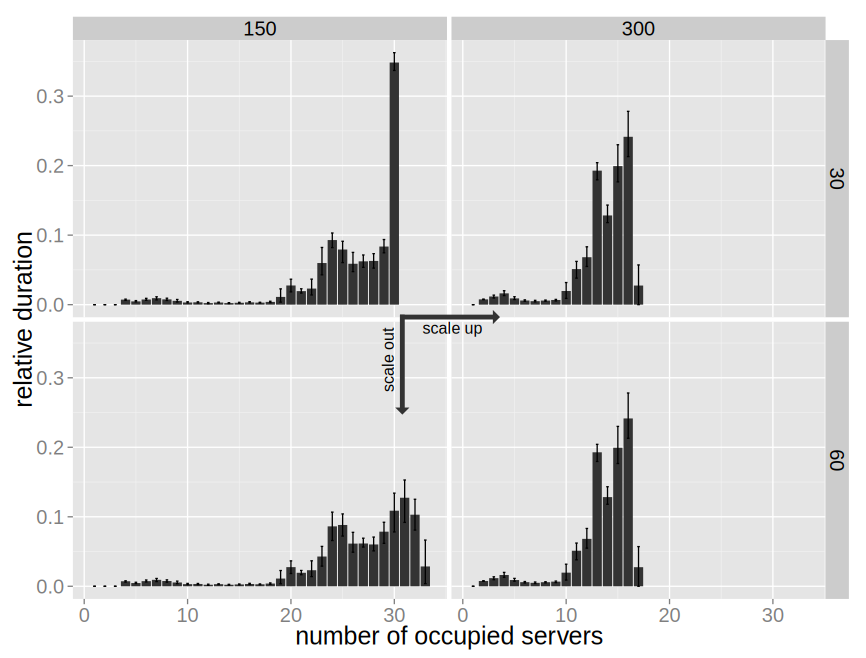
\includegraphics[width=1.0\textwidth]{images/resourceusedistribution-detail-barplot-annotated.pdf}
  \caption{Resource usage from select maximum instances and tunnels combination, displaying the capability to scale.}
 \label{c4:fig:res-usage-barplot}
\end{figure}


\begin{figure}[htb]
  \centering
  \includegraphics[width=1.0\textwidth]{images/startstopduration-blockingprobability-barchart.pdf}
  \caption{Influence of the boot and shutdown time on the blocking probability.}
 \label{c4:fig:blockprob-startstop-barchart}
\end{figure}

\begin{figure}[htb]
  \centering
  \includegraphics[width=1.0\textwidth]{images/feasiblemultiserver-blockprob.pdf}
  \caption{Comparison of the blocking probability of various server configurations.}
 \label{c4:fig:blockprob-multiserver}
\end{figure}

\begin{figure}[htb]
  \centering
  \includegraphics[width=1.0\textwidth]{images/feasiblemultiserver-blockprob.pdf}
  \caption{Comparison of the resource usage of various server configurations.}
 \label{c4:fig:res-usage-multiserver}
\end{figure}

\begin{figure}[htb]
  \centering
  \includegraphics[width=1.0\textwidth]{images/instanceuse-mean.pdf}
  \caption{Mean instance usage of various server configurations.}
 \label{c4:fig:res-instance-usage-mean}
\end{figure}



%%%%%%%%%%%%%%%%%%%%%%%%%%%%%%%%%%%%%%%%%%%%%%%%%%%%%%%%%%%%%%%%%%%%%%%%%%%%%%%
\subsection{Modeling Discussion}




%%%%%%%%%%%%%%%%%%%%%%%%%%%%%%%%%%%%%%%%%%%%%%%%%%%%%%%%%%%%%%%%%%%%%%%%%%%%%%%%
%!TEX root = ../../dissertation.tex
%%%%%%%%%%%%%%%%%%%%%%%%%%%%%%%%%%%%%%%%%%%%%%%%%%%%%%%%%%%%%%%%%%%%%%%%%%%%%%%%
\section{Measurements}
\label{c3:measurements}

With these playback models at hand, this section demonstrates how to conduct actual evaluations of reliable streaming protocols with it.

As discussed, there are numerous incarnations of reliable streaming protocols in use. Almost all of them follow the same basic approach but with slight variations in execution and choice of playback strategies and corresponding parameters. But it is exactly these choices that can have a large impact on the streaming process and resulting quality. 

The problem lies in comparing these protocols to each other. Each of them is usually tied to a specific -- and most often proprietary closed source -- streaming player. Setting up all these players in one testbed is a huge effort and requires very specific software environments to be used on the client machines. Moreover, these players are built with user interaction and not automation and directly measuring the outcome in mind. This can still be achieved through extensive workarounds, but must be tailored to every player application. The presented approach avoids this hassle and provides a concise way to test any conceivable playback strategy in one single test setup.


%%
\subsection{Progressive Streaming Measurement Framework}

To enable quick evaluations for progressive streaming the framework follows a two phase approach, separating the active online recording phase from the passive playback emulation. Recording data is very time intensive and cannot be sped up when conducting investigation of a real world process, and not relying on simulated data. It still replicates the steps a user would perform to consume a media stream on a playback device. Through appropriate configuration different scenarios can be modeled, e.g. network conditions, behavior and specifics of the user device.
 
\begin{figure}[htb]
    \includegraphics[width=\textwidth]{images/measurement-model.pdf}
    \caption{Measurement framework for progressive streaming playback strategies overview.}
    \label{c3:fig:framework}
\end{figure}

Figure \ref{c3:fig:framework} depicts the framework for a streaming evaluation testbed. In phase one the stream's transmission is conducted and recorded on a per-packet level. Stream data is transmitted to the client from a server which can be any actual streaming service on the Internet or a local server under the testbed's control, eliminating undesired side effects caused by the Internet connection. 

The traffic is directed through a network emulation node capable of altering the network \gls{QoS} parameters, i.e. latency, jitter, and packet loss. The parameters can be set according to stochastic models derived from actual network architectures. Instead of network emulation, any preexisting architecture can also be placed here to achieve more accurate results for the intended target. This is especially helpful for complex infrastructures hard to model or with no good and concise models available yet, for example mobile and mobile core networks with the influence of encapsulating traffic into bearers.

The measurement host downloads and records the video stream as a network trace. For progressive \gls{HTTP} streaming, a single request on the video file is issued and the \gls{TCP} connection maintained until the file has fully arrived.
This process is recorded as basis for the second phase. These traces should consist of the size and timestamp of every incoming packet. More detailed traces can be used to scrutinize other layers of the connection, e.g. the dynamics of TCP receive window size. Additionally the received file is decoded yielding a trace of all video frame sizes and playout timestamps.

In the second pass, these two traces are then used to feed the actual reliable streaming playback model described before. This conducted by a closed-loop emulation process calculating the current buffer fill level based on the collected transmission and video frame traces for every point in time. 

All of the progressive streaming -- i.e. non-adaptive -- strategies can be tested on the same trace set.
In simple \gls{HTTP} streaming, the transmission is not controlled by the streaming application and no rate control is conducted. Therefore, recording the packet trace and simulating playback are completely decoupled, as the latter cannot influence the former.  This enables fast and efficient comparison of non-feedback protocols subject to the same network conditions.

The emulator then generates playback stalling statistics, specifically their number and duration, to compare the effect of the different strategies on the same trace. With these results, parameter settings for playback strategies can also be iteratively tested and improved leading to an empirical calibration of playback strategies instead of relying on best practices.

One of the drawbacks of this model-based emulation approach is of course the reliance on suitable models and playback strategies for the stream protocols under scrutiny. Obtaining these from proprietary streaming clients, can be a difficult reverse-engineering process.


%%
\subsection{Adaptive Streaming Measurement Framework}

Up to this point, the measurement framework is only suitable for progressive streaming omitting any adaptive strategy. This second framework modifies this and additionally allows for the testing of adaptive playback strategies. However, to achieve this, the advantageous two phase setup cannot be employed anymore.

\begin{figure}[htb]
    \includegraphics[width=\textwidth]{images/feedback-measurement-model.pdf}
    \caption{Measurement framework for adaptive streaming playback strategies overview.}
    \label{c3:fig:framework-feedback}
\end{figure}

Figure~\ref{c3:fig:framework-feedback} shows the adapted framework. The playback emulation process is now directly fed with the stream transmission without recording it first. The emulation is now an online process and has to be conducted in realtime. This enables the emulator to react on the current streaming state and request an alteration from the server. The adaptation spectrum ranges from the timing of stream segment retrieval to the chosen quality level of future segments. 

While allow for a wider range of playback strategies, this approach is also inherently slower as it does not allow a speed-up beyond realtime, limiting its usability somewhat. Therefore, a transition to a full simulative approach is suggested. This is path is further explored and discussed in Section~\ref{c5:mobilestreamingtestbed}.

\todo{check simulation approach ref or further explain simulation}


%%
\subsection{Technical Implementation}

To conduct measurements, the described two phase progressive streaming measurement framework was implemented in a testbed. This testbed consists of three interconnected physical nodes running Linux. 

The optional streaming server houses an Apache httpd\footnote{\url{https://httpd.apache.org/}} Web server, hosting the files that are to be streamed. Alternatively, Internet streaming service traffic can also be directly routed through the network emulation node.

The network emulation node uses the existing \gls{QoS} capabilities of the Linux kernel, dubbed NetEm \cite{hemminger2005network}, to add latency and packet loss to the transmission as well as to act as a bandwidth bottleneck. The additional delay is set deterministically, the loss follows a uniform distribution without any correlation in the transmission.

To both retrieve the streaming file and record the transmission process at the client, curl\footnote{\url{http://curl.haxx.se/}} is used. If so desired, tcpdump\footnote{\url{http://www.tcpdump.org/}} can also be facilitated to achieve a higher recording precision. The video file is then parsed for its frames and sizes using mplayer\footnote{\url{http://www.mplayerhq.hu/}} with libav\footnote{\url{https://libav.org/}}. The traces are then put into the actual playback emulation, implemented by custom Python-based code and statistically evaluated with Python as well as R.



%%
\subsection{Measurement Series and Evaluations with the Framework}
%[visualization and results (does yt still work well with high delay/loss?)]
%[performance evaluation (BWs, played vs received data)]
%Also observed and analyzed. The deduce that the initial buffering time and the later block sending rate are directly correlated. 64kb blocks, probably due to GFS, problems with this method, ...
%These Quality-of-Service parameters loss and delay do not have any direct influence on the downloading process but instead have negative impacts on the throughput of the underlying TCP due to its congestion control feature and, in the end, serve as another source of delay and jitter.

This implementation has been used to conduct a comparative study of two theoretical and two real world playback strategies. They are tested for their susceptibility to worsening network \gls{QoS}, latency and loss in this case.

The video used in the experiment was streamed from the YouTube web site providing a realistic foundation for the experiments. This also enables a server side pacing mechanism adjusted to the video bitrate for free
Details on the video used in the experiment are available in Table~\ref{c3:tbl:videoparams}. Two measurement series are performed with this video, both only differ in the network emulator setting. The first series increasingly adds packet loss to the stream, with the second series altering the packet delay. 

\begin{table}[htbp]
    \centering
    \caption{Test Video Parameters}
    \label{c3:tbl:videoparams}
    \begin{tabu}{|l|X[r]|}
        \hline
        Parameter & Value \\ \hline
        Video Duration  & \SI{92.536}{\second}\\
        Size & \SI{9.61}{\mebi\byte} \\
        Framerate & \SI{23.976}{\per\second} \\
        Average Video Bitrate & \SI{871}{\kilo\bit\per\second} \\
        Codecs & AVC+AAC \\ \hline
    \end{tabu}
\end{table}


%% latency
In the latency measurement series, the emulator delayed forwarding the packets for a constant amount of time
The latency was increased in \SI{100}{\milli\second} steps, up to a total of \SI{5000}{\milli\second}. The added latency is split up evenly between the uplink and the downlink.


It can be stated, that all playback strategies will generally work very similar under good network conditions. If sufficient bandwidth is available, they will play videos with almost no delay or intermediate buffering. 
If, however, the achievable \gls{TCP} goodput is close to the average video bitrate, the buffer can be quickly drained by short deviations from the average transmission and video bit rates. The \gls{TCP} goodput can be limited by high latency and loss. Many \gls{TCP} congestion control algorithms depend on the round trip time. If the \gls{RTT} is high, the congestion window will increase much slower. High latency can also trigger \gls{TCP} timeouts and retransmissions, and in turn decrease the congestion window, further impacting the goodput. 

%% <-- WIP

The latency measurements are depicted in Figures \ref{c3:fig:eval-latency-stallingtime} and \ref{c3:fig:eval-latency-numstalls}. The stalling time increases with the additional latency. The Initial Start Delay model provides the best possible result in terms of pure stalling time. On the other hand, Figure \ref{c3:fig:eval-latency-numstalls} shows the Stalling model provides always the worst result for the number of stalls. Any other model will lie beyond that line. The Flash and HTML5 models both run in just a few buffering events which however tend to increase in length with rising latency. Attributed to the simple and optimistic assumption of the Flash model, stalling time is usually lower than with HTML5, at the cost of slightly more buffering events.
 

\begin{figure}[htb]
    \centering
    \includegraphics[width=\textwidth]{images/eval-latency-stallingtime.pdf}
    \caption{Total stalling time.}
    \label{c3:fig:eval-latency-stallingtime}
\end{figure}

\begin{figure}[htb]
    \centering
    \includegraphics[width=\textwidth]{images/eval-latency-frequency.pdf}
    \caption{Playback model observations on additional latency. Number of stalls.}
    \label{c3:fig:eval-latency-numstalls}
\end{figure}


% loss
In the loss experiment series, uncorrelated uniformly distributed loss was added in both the uplink and the downlink direction. The loss was increased in $2\%$ steps up to a total additional loss of $14\%$

TCP goodput is even more severely affected by packet loss. A lost packet results in a duplicate acknowledgement, retransmissions, and a decrease of the congestion window. The problem gets worse if also the ACKs are lost and the connection stalls on missing old segments without which the playback cannot proceed. Figure xyz shows some exemplary measurements for a loss scenario. While additional packet losses of up to four percent seem to have no noticeable impact on streaming quality, the total stalling time suffers a large increase for any model as seen in Fig. \ref{c3:fig:eval-loss-stallingtime} rendering any streaming attempts practically unusable. Figure \ref{c3:fig:eval-loss-numstalls} shows the extremity of the Stalling model compared to other models reaching a number orders of magnitude larger than any other model.
As a result, when planning a network for streaming applications, the maximum loss should be kept below the noticed mark to achieve reasonable streaming quality. 


\begin{figure}[htb]
% used yt-delay/hPUGNCIozp0_delay_100 2, spyder with matplotlib config patch
    \centering
    \includegraphics[width=\textwidth]{images/eval-loss4mb-stallingtime.pdf}
    \caption{Playback model observations on additional packet loss. Total stalling time.}
    \label{c3:fig:eval-loss-stallingtime}
\end{figure}

\begin{figure}[htb]
    \centering
    \includegraphics[width=\textwidth]{images/eval-loss4mb-frequency.pdf}
    \caption{Playback model observations on additional packet loss. Number of stalls.}
    \label{c3:fig:eval-loss-numstalls}
\end{figure}
 
 %%




For this the simple stalling model is used because this results in the shortest possible playback duration in every scenario. Furthermore, we used a network emulation testbed to subject the video streaming to increased loss and latency while fixing the maximum network bandwidth and observe the influence on the QoE.

First use case to show how our system works: Progressive HTTP streaming. Will show adaptability to adaptive streaming and different protocols. For this comparison we used a video of about \SI{90}{second} length and network conditions that could not fulfill the video bitrate in time and hereby forced stalling to occur.

We performed two measurement series, one with increased packet loss, the other one adding latency to the path. For each value of loss and latency a mean total stalling time was calculated out of five separate experiments to eliminate temporal and network load influences. Additionally, standard deviations are shown in the resulting graphs. We clearly notice very large deviations in some experiments. Some of these can be explained by connection timeouts and later resumption of the streaming. Furthermore, an exponential regression line shows the trend of the total stalling times in the experiments.




%% <-- %% end WIP

\begin{figure}[htbp]
    \centering
    \includegraphics[width=\textwidth]{images/R-delayseries.pdf}
    \caption{Total buffering time and linear smooth for degraded network parameter scenarios. Latency Graph.}
    \label{c3:fig:delayseries}
\end{figure}

\begin{figure}[htbp]
    \centering
    \includegraphics[width=\textwidth]{images/R-lossseries.pdf}
    \caption{Total buffering time and linear model for degraded network parameter scenarios. Loss Graph.}
    \label{c3:fig:lossseries}
\end{figure}

Figure \ref{c3:fig:delayseries} displays the results of of the latency measurement series with up to five seconds of additional delay. In the worst case the stalling time increases to about 50 seconds. In mobile scenarios latencies of up to 2 seconds can be expected, which would, according to our measurements, result in a maximum mean stalling time of 15 seconds for a 90 second video, which could very well be bearable for YouTube users.

There are several factors that could contribute to the increase in stalling time in the latency experiments. 
TCP, in its simplest form, increases the congestion window based on the Round Trip Time (RTT), making it highly dependent on this connection parameter. Newer congestion avoidance algorithms, e.g. the CUBIC algorithm used in Linux \cite{ha2008cubic}, however reduce this dependence on the RTT.
Another influencing factor might be YouTube's block sending mechanism, which, according to \cite{alcock2011afcyt}, may negatively interact with congestion control algorithms. The impact of packet loss on stalling is much higher than that of latency in our measurements. Yet, due to TCP's reliable transmissions, loss only causes increased packet retransmissions, and, thus, acts as a source of burst delay which negatively impacts the overall throughput.

Figure \ref{c3:fig:lossseries} shows the series of loss experiments. While the 6\% packet loss and below has an almost negligible influence on the stalling time anything above this value will probably not achieve good user experience at all. Interesting to note is the rather sudden increase in stalling time when there is more than 6\% loss added. This could again hints to the transport protocol's reliable transport feature, which catches all the occurring losses, through timeouts or gaps in the sequence numbers. However, the detection and retransmission takes some time, which is reflected in the increased stalling time.







Through these to exemplary experiments, we tried to show that network QoS parameters have a direct measurable impact on the application layer, namely on HTTP streaming quality. While the models scale rather well with latency, any HTTP streaming is almost impossible with high packet loss values.
Comparing the presented playback models, we conclude that every model represents a trade-off between several parameters, e.g. as measured here, the number and length of stalls. With the knowledge gained from the experiments, playback models could be tailor-made to best suit certain conditions and user requirements. 


%%%%%%%%%%%%%%%%%%%%%%%%%%%%%%%%%%%%%%%%%%%%%%%%%%%%%%%%%%%%%%%%%%%%%%%%%%%%%%%%


%%%%%%%%%%%%%%%%%%%%%%%%%%%%%%%%%%%%%%%%%%%%%%%%%%%%%%%%%%%%%%%%%%%%%%%%%%%%%%%%
%%%%%%%%%%%%%%%%%%%%%%%%%%%%%%%%%%%%%%%%%%%%%%%%%%%%%%%%%%%%%%%%%%%%%%%%%%%%%%%%
%%%%%%%%%%%%%%%%%%%%%%%%%%%%%%%%%%%%%%%%%%%%%%%%%%%%%%%%%%%%%%%%%%%%%%%%%%%%%%%%
\section{Summary}
\label{c3:sec:conclusion}

Streaming to mobile devices, especially in mobility scenarios, arises several new issues not seen at wireline connected devices. The lower-layer protocols on the radio link can cause additional unexpected behavior. Handover between radio cells can cause long periods of very high delay (up to seconds) and packet reordering which does not play well with TCP, resulting in a decreased throughput. Therefore, we would like to investigate its interplay with server-side bandwidth pacing methods as employed by YouTube.


We also would like to extend our analysis of video streaming to adaptive HTTP streaming mechanisms previously mentioned. We expect them to further complicate the client's buffer management algorithms but they could also serve as a full replacement and evolution to RTP streaming.


%%
In our research we analyzed both the topology as well as the streaming performance of the YouTube platform as a popular example for today's Web-based video delivery. 

With the Seattle platform we actively probed the CDN and discovered several geographical and time-dependent features. Through streaming experiments we have shown that packet loss and delay have considerable influence on the quality of the HTTP video delivery but overall it is reasonably robust to conditions in normal wireline networks. Whether they work as well in wireless networks is a question for future research. Furthermore, we looked at various theoretical and real-world buffering models. We observed that one needs to strike a balance between frequency and length of buffering phases to achieve acceptable playback quality. However, quantizing the quality is also a topic for further research.



%albeit for values which probably will not be observable in the wild for wireline network accesses and if providers have sufficient infrastuctures
% however mobile could very well ...


%% PV Conclusion
Because of rapid developments in the field of video streaming, full-scale measurement campaigns and analytical modeling might prove too time consuming to test every new protocol. The streaming model framework presented here offers methodologies to quickly evaluate new streaming mechanisms under the influence of network QoS as it decouples the network trace recording and the playback model calculation phase.

We detailed possible influences of the different network layers on video streaming, This inspired the creation of a generic model, incorporating universal notions on data transport, flow control, and buffering, striving to cover most possible streaming methods. Using this model, we explored the theoretical quality limits for streaming such as limits for the maximum stalling duration, and the user trade-offs incurred by making specific choices on how to treat conditions related to streaming processes. In our evaluation of the model on YouTube we observed the influence of network QoS on playback quality and found that high loss is detrimental to HTTP streaming.


The purpose of this model and its evaluations is manifold. It could lead to protocols tailor-made for specific networks or an improved network planning process.






%%%%%%%%%%%%%%%%%%%%%%%%%%%%%%%%%%%%%%%%%%%%%%%%%%%%%%%%%%%%%%%%%%%%%%%%%%%%%%%%%%%%%%%%%%%%%%%%%%%%

%Web-based video streaming in general

%Web, Flash, HTML5
  
%relevance for mobile and future Internet

%Drawbacks (no streaming, scaling, signaling, etc)

%Internet Load and Video delivery performing with load
  
%Example of YouTube

%Recent changes in the architecture after YouTube was acquired by Google

%applicable quality metrics (normal metrics don't apply, no video quality scaling, observable only initial buffering time, stalls during playback, number, length, frequency thereof)

%streaming-buffering-playback model creation

%Why model at all?
%Understand the problem and dissect it / break it down to its elemental components
%Find similar problems/models, extend the model for other problems

Quantification of quality of experience for edge-based applications\cite{hossfeld2007quantification}

  
%Overview on the models:
%  Generic HTML5 model:
%  "automatically begin playback of the media resource as soon as it can do so without stopping"

%  Firefox model:
%   Buffer 30 seconds of media time or do so at least for 30 seconds
%   If download bitrate greater than media bitrate then start playing immediately.
%   Exceptions apply for special cases.
    
%  Flash model:
%    Buffer at least two seconds of the media resource before starting to play. If the player has filled the 2 second buffer, the buffer size increases by another two seconds and buffering (while already playing) continues. If the buffer runs out any time during the playback the player buffers at least five seconds of the media resource before continuing.
  
%  We implemented a source model which tries to resemble these applications. We based our work on the HTML5 model as it was the simplest yet still effective, delaying the start of the playback until it can be consumed in one pass.
  
%[general observations, YouTube rate limiting, correlation to media bit-rate]
  

%[network emulation setup, degraded network quality of service parameters (netem Aufbau, delay und loss serien bei bw-begrenzung)]

%[visualization and results (does yt still work well with high delay/loss?)]

%[performance evaluation (BWs, played vs received data)]


%Also observed and analyzed. The deduce that the initial buffering time and the later block sending rate are directly correlated. 64kb blocks, probably due to GFS, problems with this method, ...


%These Quality-of-Service parameters loss and delay do not have any direct influence on the downloading process but instead have negative impacts on the throughput of the underlying TCP due to its congestion control feature and, in the end, serve as another source of delay and jitter.


